\section{密度的运算}
\label{sec:dens-rules}

有了密度以后，最常用的操作都围绕“换参考测度”：把对目标测度的积分改写成对参考测度的加权积分；把几个目标测度相对同一参考的密度组合起来；经过一个中间测度连续换两次参考；或者把参考与目标的角色对调。本节在同一可测空间$(X,\mathcal A)$上依次建立这些规则，每条规则都注明所需的测度关系，以及等式在哪个测度的几乎处处意义下成立。

\subsection{换测度的积分公式}
\label{sec:dens-change-of-measure}

密度的定义~\eqref{eq:dens-definition}只说明指示函数$\mathbf 1_A$对$\nu$的积分等于$\mathbf 1_Ah$对$\mu$的积分。积分本来就是从指示函数出发，经简单函数和单调逼近推广到一般函数的，所以这个等式可以沿同一条路线推广。

\begin{theorem}[换测度公式]
\label{thm:dens-change-of-measure}
设$\mu,\nu$是$(X,\mathcal A)$上的非负测度，$h$是$\nu$相对于$\mu$的密度，约定$0\cdot(+\infty)=0$。
\begin{enumerate}
\item 对每个可测函数$f:X\to[0,+\infty]$，
\begin{equation}
\int_Xf\,\mathrm d\nu=\int_Xfh\,\mathrm d\mu .
\label{eq:dens-change-of-measure}
\end{equation}
\item 对实值或复值可测函数$f$，$f$对$\nu$可积当且仅当$fh$对$\mu$可积，此时式~\eqref{eq:dens-change-of-measure}成立。
\end{enumerate}
\end{theorem}

\begin{proof}
(1) 对$f=\mathbf 1_A$，两边分别是$\nu(A)$与$\int_Ah\,\mathrm d\mu$，由密度的定义相等。对非负简单函数，两边对$f$都是线性的，等式成立。对一般非负可测$f$，取非负简单函数列$s_n\uparrow f$。因$h\geq0$，$s_nh$也递增并逐点收敛到$fh$。两边分别用单调收敛定理，
\[
\int_Xf\,\mathrm d\nu=\lim_{n\to\infty}\int_Xs_n\,\mathrm d\nu=\lim_{n\to\infty}\int_Xs_nh\,\mathrm d\mu=\int_Xfh\,\mathrm d\mu ,
\]
两边允许同时为$+\infty$。

(2) 对$\lvert f\rvert$用(1)，得$\int\lvert f\rvert\,\mathrm d\nu=\int\lvert fh\rvert\,\mathrm d\mu$，两种可积性等价。实值时$(fh)^\pm=f^\pm h$，对$f^+,f^-$分别用(1)，各得两个有限数，相减即得等式。复值时对实部和虚部分别处理。
\end{proof}

\term{换测度公式}（change-of-measure formula）把“对目标测度累计”改写成“对参考测度加权累计”。被积的变量与函数$f$都不变，点不移动，改变的只是每一处的累计权重。例如$[0,1]$上$\nu$相对于长度的密度为$h(x)=2x$，取$f(x)=x$，则$\int f\,\mathrm d\nu=\int_0^1x\cdot2x\,\mathrm dx=\tfrac23$；若$\nu$是概率测度，这就是用概率密度计算期望的公式。

两部分的条件不同。非负函数不需要任何可积性，等式两边可以同为$+\infty$；实值或复值函数则必须先由$\lvert f\rvert$确认两边绝对可积，否则正部与负部的积分可能都是$+\infty$，不能相减。证明中没有用到$\mu,\nu$的有限性：只要密度存在，公式就成立。

\subsection{密度的线性组合}
\label{sec:dens-linear-combination}

相对同一个参考测度，几个目标测度组合起来时，密度怎样组合？非负组合可以直接相加；带符号的组合还要先保证测度之差有定义。

\paragraph{共同参考下的非负组合}
设$\nu_1,\ldots,\nu_m$相对于同一个参考测度$\mu$分别有密度$h_1,\ldots,h_m$，$a_1,\ldots,a_m\geq0$。由非负积分的线性性，对每个可测集$A$，
\[
\sum_{i=1}^ma_i\nu_i(A)=\sum_{i=1}^ma_i\int_Ah_i\,\mathrm d\mu=\int_A\sum_{i=1}^ma_ih_i\,\mathrm d\mu ,
\]
所以$\sum_ia_i\nu_i$的密度是$\sum_ia_ih_i$。关键是参考测度相同：密度是相对于参考的换算比例，只有同一种参考下的比例才能直接相加。非负系数的可数和同样成立，此时交换求和与积分的依据是单调收敛定理。

共同参考还能把一个相对于长度没有密度的测度写成单个函数的积分。

\begin{example}[点质量与长度的统一表示]
\label{ex:dens-mixed-reference}
在$[0,1]$上取参考测度$\mu=\lambda|_{[0,1]}+\delta_0$。对可测集$A\subset[0,1]$，
\begin{equation*}
\begin{aligned}
\int_A\mathbf 1_{(0,1]}\,\mathrm d\mu&=\lambda(A\cap(0,1])+\delta_0(A\cap(0,1])=\lambda(A),\\
\int_A\mathbf 1_{\{0\}}\,\mathrm d\mu&=\lambda(A\cap\{0\})+\delta_0(A\cap\{0\})=\delta_0(A),
\end{aligned}
\end{equation*}
其中用了$\lambda(\{0\})=0$与$0\notin(0,1]$。所以$\mathrm d\lambda|_{[0,1]}/\mathrm d\mu=\mathbf 1_{(0,1]}$，$\mathrm d\delta_0/\mathrm d\mu=\mathbf 1_{\{0\}}$。由线性组合规则，$a,b\geq0$时$\nu=a\lambda|_{[0,1]}+b\delta_0$的密度是$a\mathbf 1_{(0,1]}+b\mathbf 1_{\{0\}}$。当$b>0$时$\nu$在长度零测集$\{0\}$上有正质量，整体没有Lebesgue密度；换用共同参考$\mu$后，点质量与长度质量就由一个函数统一表示。
\end{example}

例中原点处的密度值$b$不能随意改动：原点在$\mu$下质量为$1$，不是$\mu$零测集。这与长度参考不同，那里单点上的取值可以任意改变。哪些点上的密度值有意义，取决于参考测度在那里有没有质量。

\paragraph{带符号的组合}
差需要谨慎处理。若$\nu_1,\nu_2$是有限测度，则$h_1,h_2$可积，$\eta=a\nu_1-b\nu_2$（$a,b$为实数）是有限有符号测度，由可积函数积分的线性性，它的密度是可积函数$ah_1-bh_2$，与定理~\ref{thm:dens-signed}一致。对无限测度不能这样做：在$\mathbb R$上取$\nu_1=\nu_2=\lambda$，形式上$h_1-h_2=0$，可$\nu_1(\mathbb R)-\nu_2(\mathbb R)=\infty-\infty$没有定义，“$\nu_1-\nu_2$”不是在所有集合上都有值的对象。更一般地，只要对相减的两项在所考虑的每个集合上都有$\int_Ah_2\,\mathrm d\mu<\infty$，差才有意义。


\subsection{链式规则}
\label{sec:dens-chain-rule}

换算比例可以连乘：先从一种参考换到中间测度，再从中间测度换到目标。为避免与Lebesgue测度的记号冲突，本小节用$\rho$表示最底层的参考测度。

\begin{theorem}[密度的链式规则]
\label{thm:dens-chain-rule}
设$\rho,\mu,\nu$是$(X,\mathcal A)$上的$\sigma$有限非负测度，且$\nu\ll\mu\ll\rho$。则$\nu\ll\rho$，并且
\[
\frac{\mathrm d\nu}{\mathrm d\rho}=\frac{\mathrm d\nu}{\mathrm d\mu}\cdot\frac{\mathrm d\mu}{\mathrm d\rho}\qquad\rho\text{几乎处处}.
\]
\end{theorem}

\begin{proof}
由Radon–Nikodym定理取$g=\mathrm d\nu/\mathrm d\mu$与$k=\mathrm d\mu/\mathrm d\rho$。对任意可测集$A$，先用$g$的定义，再对非负函数$\mathbf 1_Ag$与密度$k$使用换测度公式，
\[
\nu(A)=\int_X\mathbf 1_Ag\,\mathrm d\mu=\int_X\mathbf 1_Agk\,\mathrm d\rho .
\]
所以$gk$是$\nu$相对于$\rho$的一个密度，由定理~\ref{thm:dens-weighted-measure}得$\nu\ll\rho$。$\nu,\rho$都$\sigma$有限，由Radon–Nikodym定理的唯一性，任何版本的$\mathrm d\nu/\mathrm d\rho$都与$gk$在$\rho$几乎处处意义下相等。
\end{proof}

这条\term{密度的链式规则}（chain rule for densities）与一元微积分的链式法则形式相似，依据却是换测度公式，而不是对坐标求导。逐次换参考与直接换参考给出同一个积分表示：对非负$f$，$\int f\,\mathrm d\nu=\int fg\,\mathrm d\mu=\int fgk\,\mathrm d\rho$。数值例子：$[0,1]$上$\rho=\lambda|_{[0,1]}$，$\mathrm d\mu/\mathrm d\rho=2x$，$\mathrm d\nu/\mathrm d\mu=\tfrac32x$，链式规则给出$\mathrm d\nu/\mathrm d\rho=3x^2$。直接核对：$\mu([0,1])=\int_0^12x\,\mathrm dx=1$，$\nu([0,1])=\int_0^1\tfrac32x\cdot2x\,\mathrm dx=\int_0^13x^2\,\mathrm dx=1$。图~\ref{fig:dens-chain-rule}画出了两段换算。

\begin{figure}[!htbp]
  \centering
  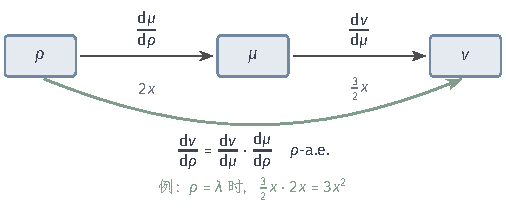
\includegraphics[width=85.651mm]{figures/02-abstract-mathematics/01-metric-and-measure/tikz/c4-chain-rule/figure.pdf}
  \caption{密度的链式规则。箭头表示“箭头终点的测度相对于起点测度的密度”：先从$\rho$换到$\mu$，再从$\mu$换到$\nu$，两段密度相乘就是从$\rho$直接换到$\nu$的密度（绿色弧线），等式在$\rho$几乎处处意义下成立。箭头下方是$[0,1]$上$\rho=\lambda$时的例子，$2x$与$\tfrac32x$相乘得到$3x^2$。}
  \label{fig:dens-chain-rule}
\end{figure}

\paragraph{各因子的几乎处处意义}
$g=\mathrm d\nu/\mathrm d\mu$只确定到$\mu$零测集，而结论是关于$\rho$零测集的。两者并不冲突。设$g'$是$g$的另一个版本，$g\neq g'$只发生在某个$\mu$零测集$M$上，于是乘积$gk$与$g'k$只可能在$M\cap\{k>0\}$上不同。由$0=\mu(M)=\int_Mk\,\mathrm d\rho$，$k$在$M$上$\rho$几乎处处为零，所以$\rho(M\cap\{k>0\})=0$。也就是说，在$k=0$处乘积按约定取$0$，与$g$的取值无关；在$k>0$处，$\mu$的零测例外也是$\rho$的零测例外。无论选哪个版本，乘积都给出同一个$\rho$几乎处处确定的密度。

\subsection{倒数规则}
\label{sec:dens-inverse-rule}

若两个测度相互绝对连续，就可以从任一方换到另一方。反向的密度应当是原密度的倒数，但这需要先保证原密度几乎处处既不为零也不为无穷。

\begin{theorem}[密度的倒数]
\label{thm:dens-inverse}
设$\mu,\nu$是$(X,\mathcal A)$上的$\sigma$有限非负测度，$\nu\ll\mu$且$\mu\ll\nu$，$h=\mathrm d\nu/\mathrm d\mu$。则$0<h<\infty$在$\mu$几乎处处成立，并且
\[
\frac{\mathrm d\mu}{\mathrm d\nu}=\frac1h ,
\]
等式在$\mu$几乎处处意义下成立，也在$\nu$几乎处处意义下成立。
\end{theorem}

\begin{proof}
由Radon–Nikodym定理可取有限值的$h$。令$Z=\{h=0\}$，则$\nu(Z)=\int_Zh\,\mathrm d\mu=0$，由$\mu\ll\nu$得$\mu(Z)=0$，所以$0<h<\infty$在$\mu$几乎处处成立。令$u=1/h$于$X\setminus Z$，$u=0$于$Z$。对任意可测集$A$，由换测度公式，
\[
\int_Au\,\mathrm d\nu=\int_X\mathbf 1_Auh\,\mathrm d\mu=\mu(A\setminus Z)=\mu(A),
\]
所以$u$是$\mu$相对于$\nu$的密度。两个测度等价，零测集相同，因此$\mu$几乎处处与$\nu$几乎处处是同一回事。
\end{proof}

这个结论也可以从链式规则读出：对$\mu\ll\nu\ll\mu$用定理~\ref{thm:dens-chain-rule}，得$(\mathrm d\mu/\mathrm d\nu)\cdot h=\mathrm d\mu/\mathrm d\mu=1$。例如$[0,1]$上$\nu$相对于$\lambda$的密度为$2x$，它只在零测集$\{0\}$上为零，所以$\nu$与$\lambda|_{[0,1]}$等价，反向密度为$1/(2x)$，$x\in(0,1]$。反向密度无界，但仍满足$\int_0^1\frac1{2x}\cdot2x\,\mathrm dx=1=\lambda([0,1])$。

\paragraph{单向绝对连续时的信息丢失}
若只有$\nu\ll\mu$，密度$h$可以在一个正$\mu$测度的区域上为零。取$\mu=\lambda|_{[0,2]}$，$\nu=\lambda|_{[0,1]}$，则$h=\mathbf 1_{[0,1]}$。在正密度区域$\{h>0\}=[0,1]$上，反向表示仍然成立：对$A\subset\{h>0\}$，$\mu(A)=\int_A(1/h)\,\mathrm d\nu$。但在零密度区域$(1,2]$上，$\mu$有质量$1$，$\nu$却为零，无论用什么函数加权，$\int_{(1,2]}u\,\mathrm d\nu$都是$0$，不可能恢复$\mu((1,2])=1$。这时$\mu$并不相对于$\nu$绝对连续，整体的反向密度不存在。图~\ref{fig:dens-one-sided-loss}显示了这块被目标测度完全忽略的区域。

\begin{figure}[!htbp]
  \centering
  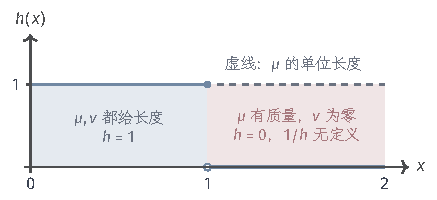
\includegraphics[width=73.914mm]{figures/02-abstract-mathematics/01-metric-and-measure/tikz/c4-one-sided-loss/figure.pdf}
  \caption{单向绝对连续时密度不能取倒数。参考测度$\mu$是$[0,2]$上的长度，目标测度$\nu$是$[0,1]$上的长度，密度$h=\mathbf 1_{[0,1]}$（蓝色实线）。在$[0,1]$上$h=1$，两种测度一致；在红色区域$(1,2]$上$h=0$，$\mu$有质量$1$而$\nu$没有质量，从$\nu$出发无法恢复这部分质量。}
  \label{fig:dens-one-sided-loss}
\end{figure}

一般地，若$\nu\ll\mu$且都$\sigma$有限，令$P=\{h>0\}$，同样的计算给出$\mu(A\cap P)=\int_A\mathbf 1_P/h\,\mathrm d\nu$，即$1/h$是$\mu|_P$相对于$\nu$的密度。原参考测度在零密度区域$X\setminus P$上的质量$\mu|_{X\setminus P}$与$\nu$相互奇异，这正是$\mu$相对于$\nu$的Lebesgue分解中的奇异部分，不能通过相除恢复。倒数公式只能在两个测度等价的范围内整体使用。
